\subsection{Low Level Design}

The low-level design explains the details of two modules; one is the interceptor module, and other is the sampling broker module.

\subsubsection{Interceptor Module}

Figure \ref{figures:artemis_interceptor} shows the class diagram for the interceptor module. The interceptor is named as Sampling Broker Interceptor. The Sampling Broker Interceptor is an incoming interceptor [\ref{subsubsection:in_interceptor}].

\makeatletter
\setlength{\intextsep}{20pt}
\makeatother

\begin{figure}[h!]
\centering
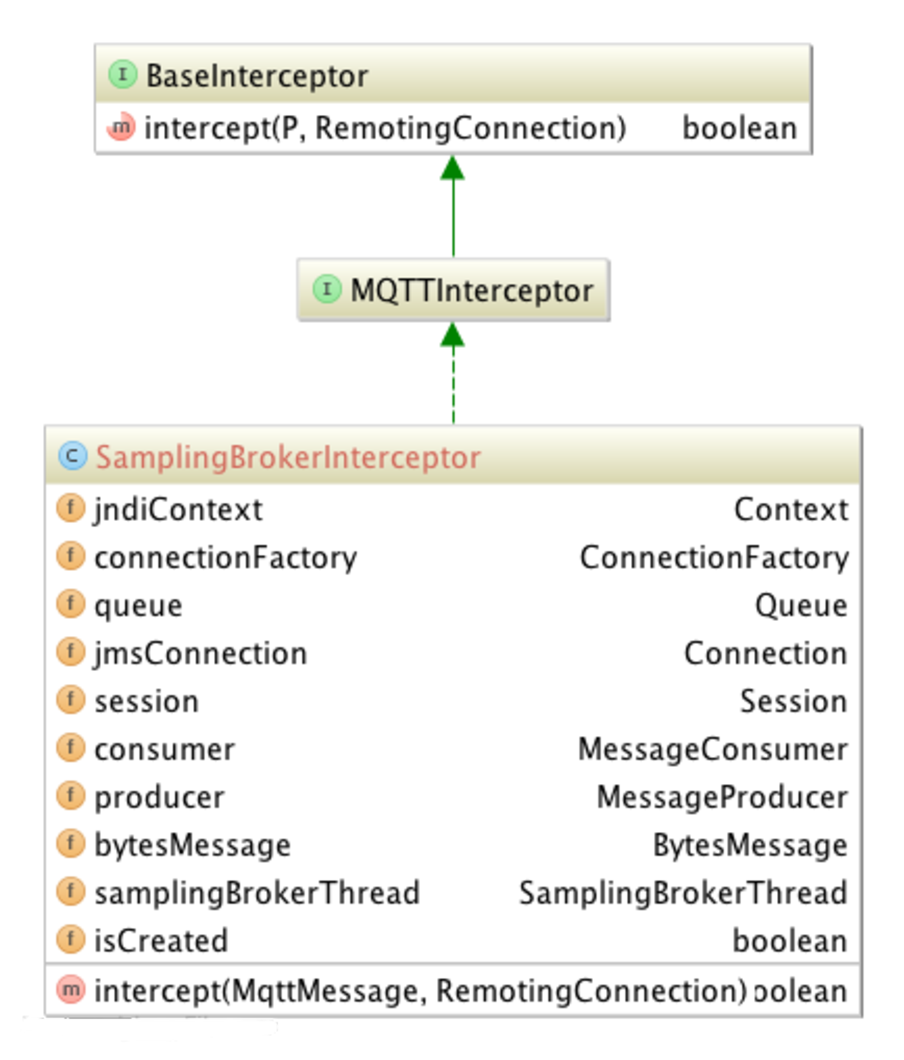
\includegraphics[keepaspectratio, width=0.6\textwidth, trim={0 0 0 0},clip]{interceptor.pdf}
\caption{Sampling Broker Interceptor Class Diagram}\label{figures:artemis_interceptor}
\end{figure}

The Sampling Broker Interceptor implements the MQTT Interceptor interface which enables it to receive all the incoming MQTT packets. The interceptor module sends the intercepted messages to a JMS queue using JMS.

\subsubsection{Sampling Broker Module}

Figure \ref{figures:artemis_thread} shows the class diagram of the sampling broker module.

\makeatletter
\setlength{\intextsep}{20pt}
\makeatother

\begin{figure}[h!]
\centering
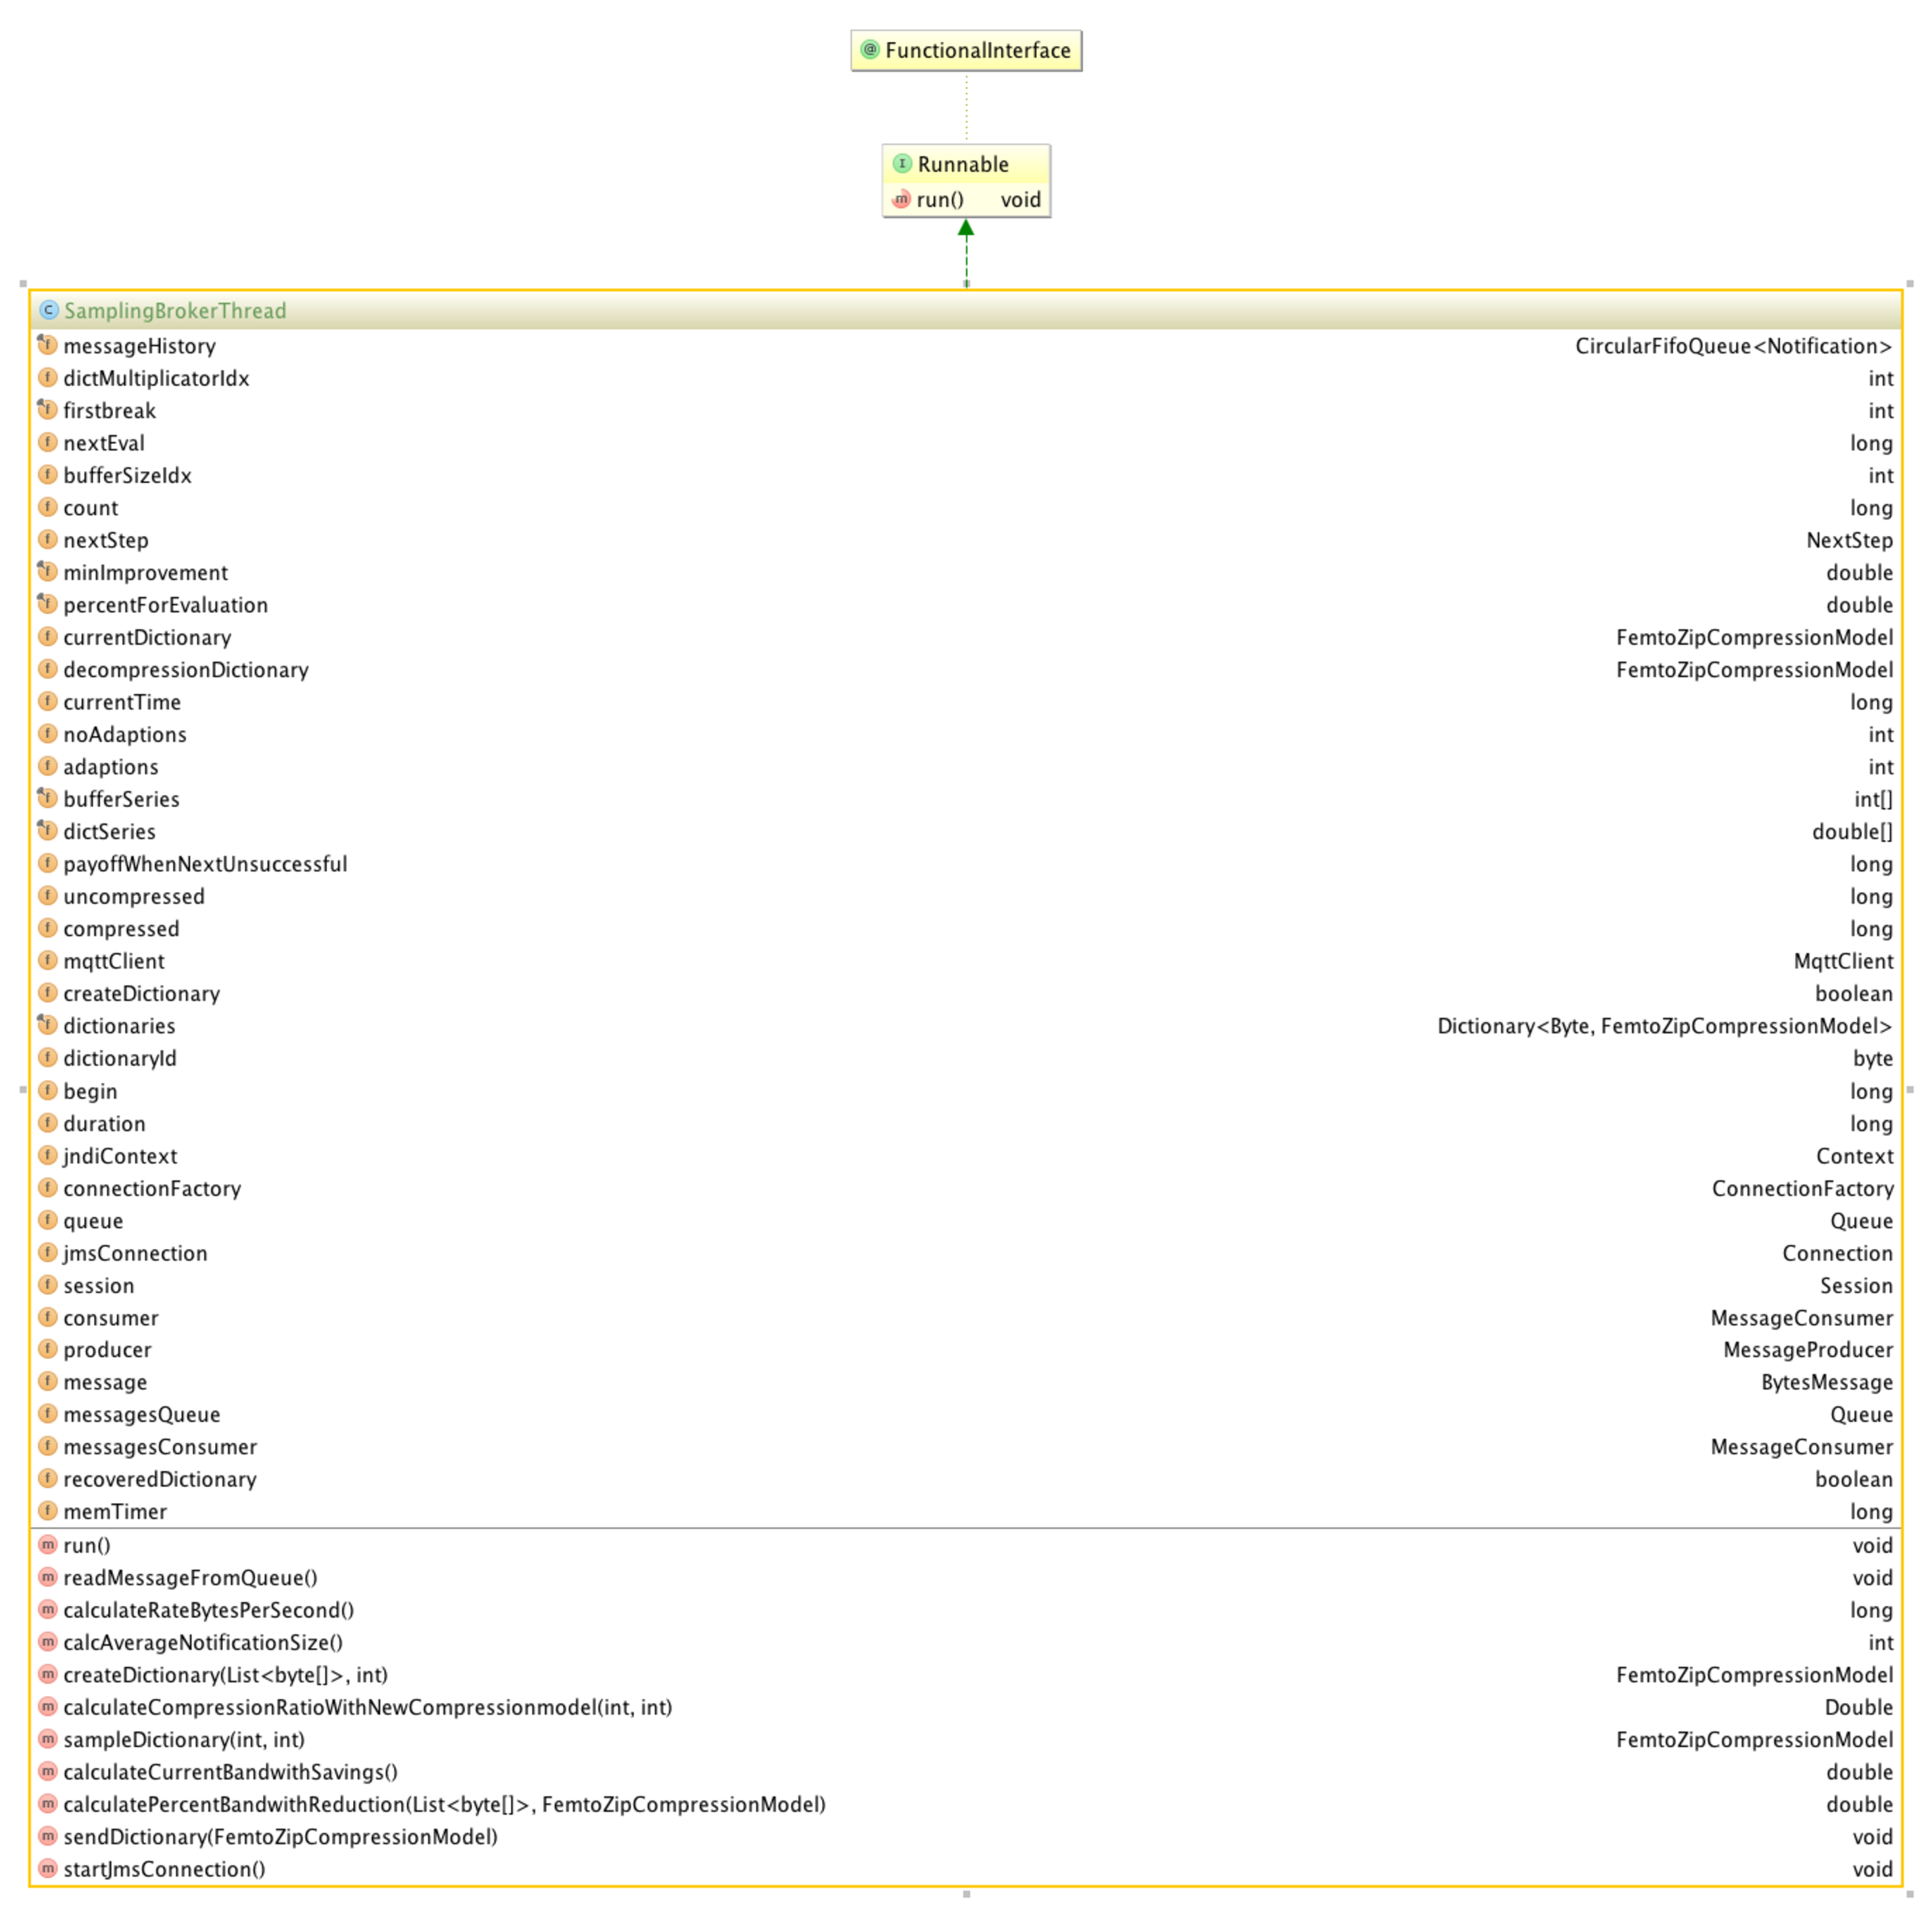
\includegraphics[keepaspectratio, width=1.0\textwidth, height=1.2\textheight, trim={0 0 0 0},clip]{thread.pdf}
\caption{SSPS for Apache ActiveMQ Artemis High Level Design}\label{figures:artemis_thread}
\end{figure}

The sampling broker runs the adaptive sampling algorithm described in the section [\ref{subsection:algo}]. The sampling broker module gets the messages from a JMS queue via JMS.

The interaction between the interceptor module and the sampling broker module is explained in detail in section [\ref{subsection:interact}].